\documentclass[letterpaper,10pt]{article}

\usepackage{enumitem}
\usepackage{titling}
\usepackage{listings}
\usepackage{url}
\usepackage{hyperref}
\usepackage{setspace}
\usepackage{subfig}
\usepackage{sectsty}
\usepackage{pdfpages}
\usepackage{colortbl}
\usepackage{multirow}
\usepackage{multicol}
\usepackage{relsize}
\usepackage{amsmath}
\usepackage{wasysym}
\usepackage{fancyvrb}
\usepackage[yyyymmdd]{datetime}
\usepackage{amsmath,amssymb,amsthm,graphicx,xspace}
\usepackage[titlenotnumbered,noend,noline]{algorithm2e}
\usepackage[compact]{titlesec}
\usepackage{XCharter}
\usepackage[T1]{fontenc}
\usepackage[scaled]{beramono}
\usepackage[normalem]{ulem}
\usepackage{booktabs}
\usepackage{tikz}
\usetikzlibrary{arrows,automata,shapes,trees,matrix,chains,scopes,positioning,calc}
\tikzstyle{block} = [rectangle, draw, fill=blue!20,
text width=2.5em, text centered, rounded corners, minimum height=2em]
\tikzstyle{bw} = [rectangle, draw, fill=blue!20,
text width=4em, text centered, rounded corners, minimum height=2em]

\definecolor{namerow}{cmyk}{.40,.40,.40,.40}
\definecolor{namecol}{cmyk}{.40,.40,.40,.40}
\renewcommand{\dateseparator}{-}

\let\LaTeXtitle\title
\renewcommand{\title}[1]{\LaTeXtitle{\textsf{#1}}}

\lstset{basicstyle=\footnotesize\ttfamily,breaklines=true}

\newcommand{\handout}[5]{
	\noindent
	\begin{center}
		\framebox{
			\vbox{
				\hbox to 5.78in { {\bf ECE 350: Real-Time Operating Systems } \hfill #2 }
				\vspace{4mm}
				\hbox to 5.78in { {\Large \hfill #4  \hfill} }
				\vspace{2mm}
				\hbox to 5.78in { {\em #3 \hfill \today} }
			}
		}
	\end{center}
	\vspace*{4mm}
}

\newcommand{\lecture}[3]{\handout{#1}{#2}{#3}{Lecture#1}}
\newcommand{\tuple}[1]{\ensuremath{\left\langle #1 \right\rangle}\xspace}

\newcommand{\Rplus}{\protect\hspace{-.1em}\protect\raisebox{.35ex}{\smaller{\smaller\textbf{+}}}}
\newcommand{\Cpp}{\mbox{C\Rplus\Rplus}\xspace}


\addtolength{\oddsidemargin}{-1.000in}
\addtolength{\evensidemargin}{-0.500in}
\addtolength{\textwidth}{2.0in}
\addtolength{\topmargin}{-1.000in}
\addtolength{\textheight}{1.75in}
\addtolength{\parskip}{\baselineskip}
\setlength{\parindent}{0in}
\renewcommand{\baselinestretch}{1.5}
\newcommand{\term}{Spring 2023}
\newcommand{\termnumeric}{1235}

\singlespace


\begin{document}

\lecture{ 20 --- More About Input/Output Devices }{\term}{Jeff Zarnett}

\section*{Transforming I/O Requests to Hardware Operations}

In the previous section we discussed the idea of taking a command like \texttt{read} and said it is the job of the device driver to translate this command into a hardware operation. Reading from the file system on disk, for example, requires a few steps. If I want to open a file like \texttt{example.txt}, the file system (not yet discussed) will associate this file with some information about where on the disk this is (a set of disk blocks representing the file). Then, to read the file, \texttt{read} commands can be issued to get those blocks into memory so I can edit it with \texttt{vi}.

The diagram below shows the life cycle of an I/O request:

\begin{center}
	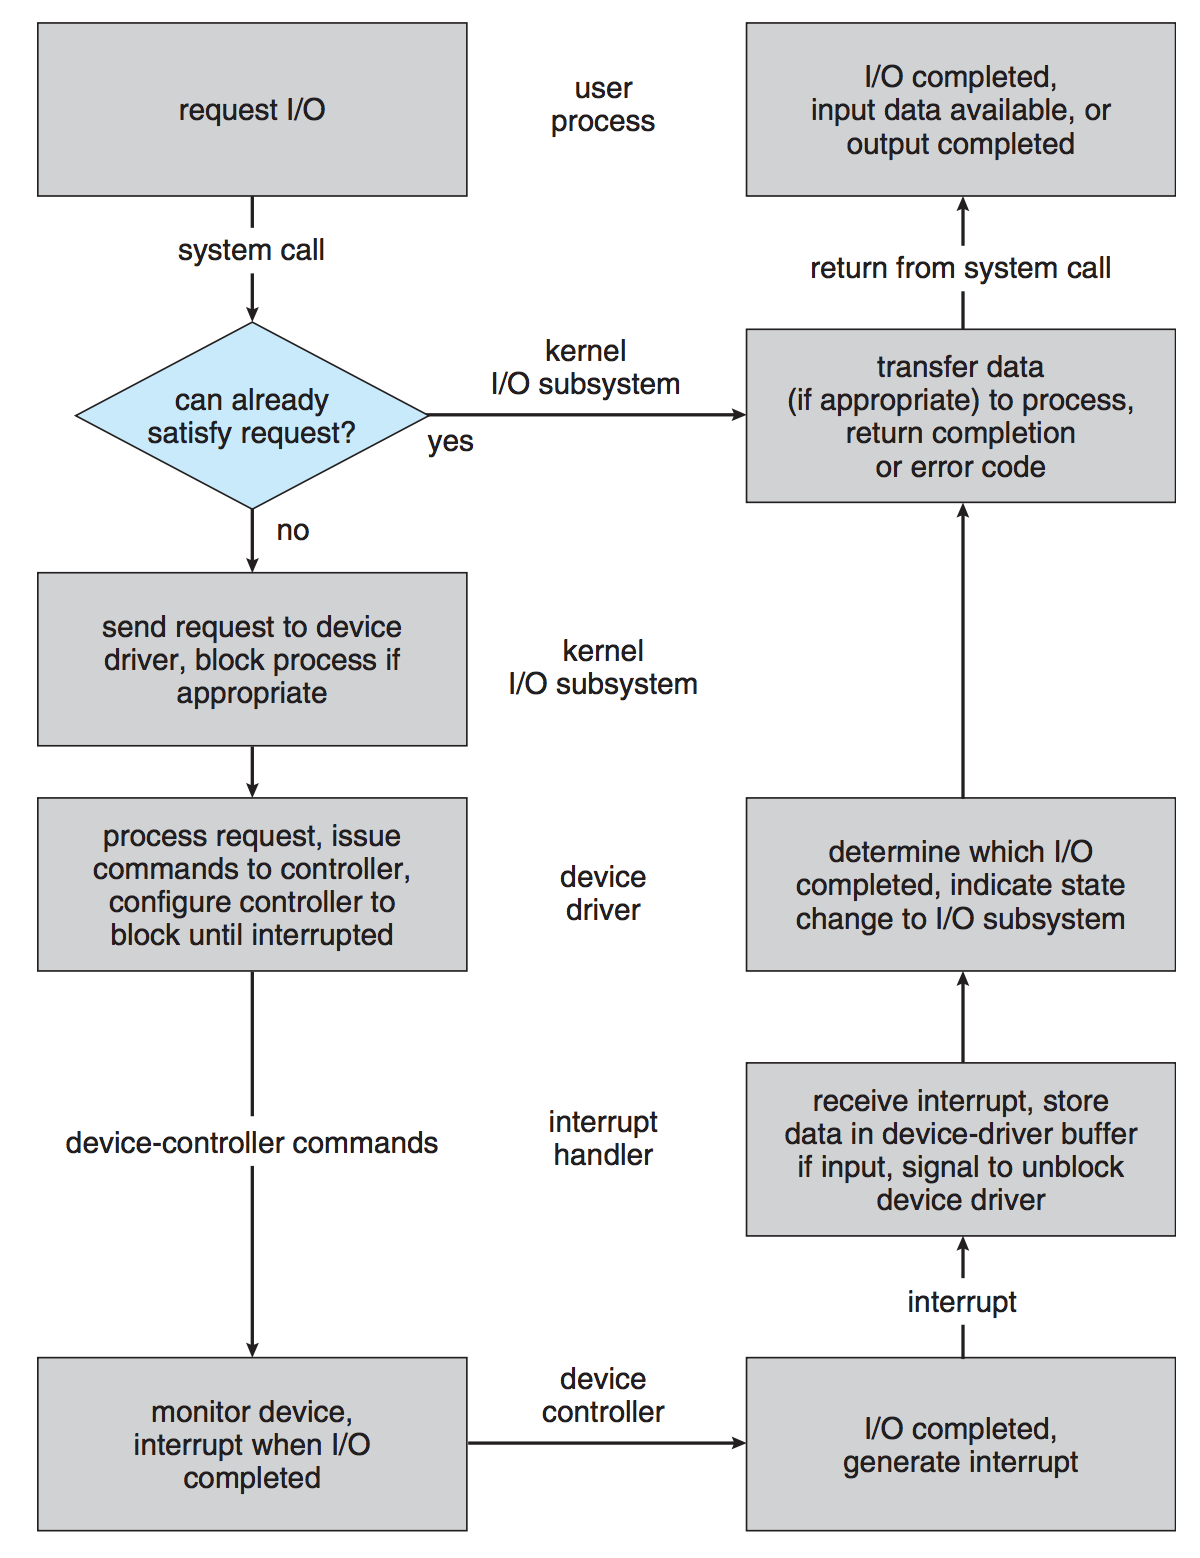
\includegraphics[width=0.65\textwidth]{images/io-lifecycle.png}\\
	The life cycle of an I/O request~\cite{osc}.
\end{center}

In general, the life cycle follows some ten steps from start to finish~\cite{osc}:

\begin{enumerate}
	\item A process issues a \texttt{read} command (assume the file is already open).
	\item The system call routine checks the parameters for correctness. If the data is in a cache or buffer, return it straight away.
	\item Otherwise, the process is blocked waiting for the device and the I/O request is scheduled. When the operation is to take place, the I/O subsystem tells the device driver.
	\item The device driver allocates a buffer to receive the data. The device is signalled to perform the I/O (usually by writing into device-control registers or sending a signal on a bus).
	\item The device controller operates the hardware to do the work.
	\item The driver may poll for status, await the interrupt when finished, or for the DMA controller to signal it is finished.
	\item The interrupt handler receives the interrupt and stores the data; it then signals the device driver to indicate the operation is done.
	\item The device driver identifies what operation has just finished, determines the status, and tells the I/O subsystem it is done.
	\item The kernel transfers the data (or error code or whatever) to the address space of the requesting process, and unblocks that process.
	\item When the scheduler chooses that process, it resumes execution.
\end{enumerate}

\section*{Buffering}

Regardless of whether a device is block- or character-oriented, the operating system can improve its performance through the use of buffering. A buffer is nothing more than an area of memory that stores data being transferred, whether it is from memory to a device, device to memory, or device to device.  A buffer is a good way to deal with a speed mismatch between devices.

You may be familiar with the idea of buffering from something like watching an online video. If each piece of the video is delivered from the server to your computer exactly when it's needed, even a small slowdown or hiccup in your network connection results in the video pausing or stuttering until the next chunk arrives. To have a smoother experience for the viewer, the video player most likely gets and stores the next few chunks a bit in advance, so if there is some temporary delay in getting a chunk then the playback is not interrupted.

The video player example is simple and familiar, but it covers all the important parts. We need a place to store the data temporarily to decouple the producing (sending from the server) and consuming (playing the video). It requires some decisions about how big the buffer should be. Bigger is not always better, mind you: if the video player wants to have $n$ chunks before starting the video, then as $n$ grows, it delays the start of playing the video. If $n$ is too large users are frustrated because the video does not start playing for a long time. The other reason is that some extra, unnecessary work will be done: if the viewer starts the video but then decides to skip forward 30\%, the player will have downloaded some chunks that were not needed. If you have a very fast internet connection, maybe this doesn't matter very much because the costs are low.

The following calculation is crude, but it does illustrate at least a little bit the performance impact of a buffer, from~\cite{osi}: We'll say $T$ is the time required to input one block and $C$ is the computation time between input requests. With no buffer, the execution time to complete a block is $T+C$; with a buffer it is max$(C, T) + M$, where $M$ is the time to move the data from a system buffer to process memory.

A buffer is usually created with a bounded capacity: the buffer can hold $x$ bytes of data and once that buffer is full, nothing else can fit in it right now so there's choices to make: either the source of data can be blocked until space is available, or older data can be overwritten with the newer data. Sometimes books talk about unbounded capacity, where the queue length can be infinite, but that's just an illusion. The memory space of the system where the data is to be stored is not infinite, even if it can seem so big that it appears to be unlimited. At some point, space \textit{will} run out, even if it's after 30 Terabytes, and then we have the same problem as the bounded buffer size: what do we do when it's full? Tempting as it is to not handle that situation, probably we should.

\paragraph{Implementing a Buffer.}
Actually implementing a buffer is relatively straightforward operation from the point of view of the operating system because it really only requires two operations: add something to and remove something from the buffer. The implementation looks exactly like the producer-consumer problem covered in a certain prerequisite course. Here's the pseudocode version of it that you might be tired of seeing:


\begin{multicols}{2}
	\textbf{Producer}\vspace{-2em}
	\begin{verbatim}
	 1. [produce item]
	 2. wait( spaces )
	 3. wait( mutex )
	 4. [add item to buffer]
	 5. post( mutex )
	 6. post( items )
  \end{verbatim}
	\columnbreak
	\textbf{Consumer}\vspace{-2em}
	\begin{verbatim}
	 1. wait( items )
	 2. wait( mutex )
	 3. [remove item from buffer]
	 4. post( mutex )
	 5. post( spaces )
	 6. [consume item]
  \end{verbatim}
\end{multicols}
\vspace{-2em}

The important thing to note is that the use of the mutex and semaphore will block and unblock threads as necessary when the buffer is full, busy, or empty. We already covered earlier in the course the implementation of those constructs so there's no need to revisit that. You may also choose to use the simpler version without the mutex if there's only one producer and one consumer.

\paragraph{Double Buffering and Circular Buffering.} Users type very slowly, from the perspective of the computer, and if we're writing to a file, it would be awfully inefficient to ask the disk, a block oriented device, to update itself on every single character. It is much better if we wait until we have some certain amount of data (e.g., a whole line or whole block or full buffer, whichever it is) and then write this out to disk all at once.

The write is, however, not instantaneous and in the meantime, the user can still keep typing. Thus, to solve this, the typical solution is \textit{double buffering}, that is, two buffers. While buffer one is being emptied, buffer two receives any incoming keystrokes. Double buffering decouples the producer and consumer of data, helping to overcome speed differences between the two~\cite{osc}.

The obvious extension beyond having two buffers is having more than two, so $n$ buffers. In that case, it's referred to as circular buffering, with each individual buffer being one of many in the circular buffer~\cite{osi}.


\paragraph{Not Magic.}
Buffering, is, however, not capable of solving all problems. If the rate at which the buffer or buffers is/are being filled consistently exceeds the rate at which the  buffer or buffers is/are being emptied, at some point the buffers will be full. When that happens, the producer side is going to get blocked until such time as space is available. The converse also applies: if the buffers are being emptied much faster than they are being filled then the consumer side will get blocked instead. Buffering does help to smooth out the peaks and valleys in the speed of these, but only up to a certain point.


\section*{I/O Scheduling and Performance}

There are potentially multiple I/O requests in progress at a time, so the operating system will need to keep track of these I/O requests in some sort of device-status table that contains an entry for each I/O device~\cite{osc}. Like we talked about for, say, a semaphore, the OS needs to keep track of the device status and also have an associated queue where threads that are blocked for that device are waiting.

Managing that queue looks significantly similar to concepts we've already examined. When a thread wants to use the device, check the device status: if it's available then we can mark the device as busy and submit the request to the device. Until the operation is complete, mark the requesting thread as blocked. If a thread shows up and wants to use a device that's already in use, just block it and add that thread to the queue. When the operation is complete, unblock the thread waiting for it and let it continue. If there are no further requests waiting, mark the device as idle (not in use). Otherwise, keep the status as busy and begin the next request.

This scheme is going to be first-come-first-served and in the discussion of how to implement a semaphore or mutex, that was typically adequate as an approach. It's very fair, but maybe not optimal. We learned in discussing scheduling that sometimes things like priorities matter more than absolute fairness.

We sometimes want to schedule I/O requests differently because I/O devices may have non-uniform access times. Many devices do have uniform access times: if we're reading a file off a USB flash drive, it doesn't matter where on the drive the drive the data is physically located. That's not true for all devices. And when it's not, it matters for the sake of efficiency.

The efficiency part is easy to motivate if we refer back to the diagram discussing the speed of various devices. I/O devices are very slow compared to the CPU so anything that uses the slow device more efficiently will speed up the execution of the system significantly.

A simple analogy: Imagine you need to go to the grocery store, the dry cleaners, and the bank. The bank is located 1~km to the west of your current location, and the grocery store is 3~km west. The dry cleaners is in the same plaza as the grocery store. It is obvious that it would be fine to go to the bank, then the dry cleaners, then the grocery store, but not to go to the dry cleaners, then the bank, then the grocery store. The unnecessary back-and-forth wastes time and energy (whether walking or fuel depends on your mode of transportation).

Clearly, the operating system will want to avoid wasting effort with I/O requests. It will maintain a structure of requests and can then re-arrange them to be accomplished most efficiently. The literature sometimes refers to this as a queue but... is it really a queue when it does not exhibit the first-in, first-out behaviour? 

This will, naturally, have some limits: requests should presumably get scheduled before too much time has elapsed even if it would be ``inconvenient''. It might also take priority into account, dealing with the I/O requests of a high priority process even if they are not particularly nearby to other requests. Like what we've discussed around scheduling, there are tradeoffs necessary to balance utilization and fairness. In particular, this is important when examining hard disk drive operation. And that will therefore be the next subject we will consider (but in the next course topic). 

\paragraph{Can a System Be Too Responsive?}
We've discussed the idea already that interrupts are more efficient than polling, you might question if there's such a thing as too responsive. Network traffic, for example, may be the cause of a lot of interrupts and a very high rate of context switches~\cite{osc}.

For downloading a file, say, the number of interrupts is probably manageable: as each chunk arrives, the interrupt is triggered, and the chunk is handled. Eventually, all the file is downloaded and there we are. That's not the scenario of concern; the scenario of concern is what happens if I use \texttt{ssh} to log in to one of the ECE servers and then use \texttt{vim} to open the C file I plan to work on.

Every time I type a character on my keyboard, a keyboard interrupt takes place, the kernel handles it, sends it to the user process (\texttt{ssh} client), which then wants to send it to the remote system. To do so, it uses a network I/O system call to send it and it goes out to the remote system. The remote system gets an interrupt on the arrival of the packet and it handles it by delivering it to the appropriate process (\texttt{vim}). And then \texttt{vim} will process the keypress and add the letter to what I'm typing. But it then updates the screen so another network request is generated from the remote machine and sent back to mine, where another interrupt is generated and has to be handled to update the view on my screen~\cite{osc}. That's a lot of system calls every time I press a key. I personally don't type super quickly from the point of view of the computer system, but imagine it's the day an assignment is due and a hundred people are using the system.

How to address that, then? In the book there are two approaches that I would describe as somewhat questionable. The first one is the idea of having the \texttt{sshd} program (well, the book says \texttt{telnet} but let's not revisit ancient history... this time) run in kernel mode so there are fewer switches. That's kind of risky, if you ask me... The other thing suggested is having some sort of specialized hardware to handle terminal connections, some sort of specific-purpose CPU to handle this sort of workload. That's weird too, because we typically do not want to buy specialized hardware just because we log into the box remotely, right? But on the other hand, there are situations where we have worked with special-purpose hardware.

Things like the translation lookaside buffer were a specific example of taking logic that was in software and moving it to hardware to make it faster. For complex devices, including hard drives, some logic will be pushed to the actual device itself, which can speed up the operations and simplify the operating system's interaction with the device. There is a cost in terms of money, of course, because more hardware on the device costs more money. It's also harder to fix any issues that are discovered because it may be expensive or impossible to fix the hardware bug. Sometimes such a hardware bug can be worked around in software, but that may undo the performance benefit of shifting it to hardware in the first place.

Other solutions look like reducing the amount of time it takes to handle an interrupt, waiting until a bigger chunk of data has arrived (or a time limit reached), or make use of DMA hardware to reduce the involvement of the CPU in moving the data around. Those might actually be plausible for the majority of scenarios.


\section*{Security}
As device drivers run at a high level of trust in the operating system, they offer an easy route for attackers to be able to get access they are not supposed to have. If a driver allows for privilege escalation or snooping the data of another process, attackers will make use of it. Let's consider an examination of a malware technique called BYOVD -- Bring Your Own Vulnerable Driver, which is nothing new having been around since at least 2012. The source for this is~\cite{byovd}.

Of course, the vulnerable driver has to be on the target system in the first place. If an administrator wishes, they can intentionally install a driver with a known vulnerability to be able to do something bad. But operating system design can't really defend against this sort of thing because the attacher is already a system administrator so they can already do bad things in other ways. 

In principle, bad drivers should not get installed automatically because of driver signing that we talked about earlier on. So a deliberately-malicious driver is unlikely to get past the validation process and the seal of approval. Trying to install a driver that's not signed tends to result in the operating system throwing a ton of warnings to say please be sure you want to do this...

Ah, but this doesn't solve the problem of what happens if there's a vulnerability in an otherwise-legitimate driver. Such a driver would have been tested, approved, and signed and the problem is only discovered after the driver is released. If a fix is prepared and published -- and that is a big if sometimes -- then anyone who installs the new version is fine (even if not everyone installs patches). But that doesn't prevent installing the old version with the vulnerability.

What is needed is some idea of revocation: a previously-approved driver should be possible to un-approve in some way so that the OS won't allow the vulnerable version to be used. The article reveals that Microsoft has not been properly applying updates to the driver block-list which resulted in exploitable drivers being installed. Oops!

Microsoft did address this once it was reported, but a little late: there were some known cases of actual exploits taking place using drivers in the block-list. And as you may imagine, the installation rate for patches to any operating system is never 100\%, so vulnerable systems will continue to exist...

\bibliographystyle{alphaurl}
\bibliography{350}


\end{document}